\documentclass{article}
\usepackage[utf8]{inputenc}
\usepackage{fullpage}
\usepackage {setspace}
\usepackage[hang,flushmargin]{footmisc} %control footnote indent
\usepackage{url} % for website links
\usepackage{amssymb,amsmath}%for matrix
\usepackage{graphicx}%for figure
\usepackage{appendix}%for appendix
\usepackage{float}
\floatstyle{plaintop}
\restylefloat{table}
\usepackage{multirow}
\usepackage{longtable}
\usepackage{morefloats}%in case there are too many float tables and figures
\usepackage{caption}
\usepackage{subcaption}
\captionsetup[subtable]{font=normal}
\usepackage{color}
\usepackage{hyperref}
\usepackage[round]{natbib}
\usepackage{appendix}
\usepackage{listings}
\usepackage{courier}
\usepackage{color}
\usepackage{setspace}
\usepackage{algorithm}
\usepackage{algorithmicx}
\usepackage[noend]{algpseudocode}
\usepackage{rotating} % rotate table by some degree
\usepackage{rotfloat}
\usepackage{mwe}
\usepackage{morefloats}
\usepackage{caption}
\usepackage{subcaption}
\captionsetup[subtable]{font=normal}
\usepackage{listings}

%\definecolor{codegreen}{rgb}{0,0.6,0}
\definecolor{codegray}{rgb}{0.5,0.5,0.5}
\definecolor{codepurple}{rgb}{0.58,0,0.82}
\definecolor{backcolour}{rgb}{0.95,0.95,0.92}
\definecolor{codeblack}{rgb}{0,0,0}

\lstdefinestyle{mystyle}{
    %backgroundcolor=\color{backcolour},
    commentstyle=\color{codegray},
    keywordstyle=\color{codeblack},
    numberstyle=\tiny\color{codegray},
    stringstyle=\color{codeblack},
    basicstyle=\normalsize\ttfamily,
    breakatwhitespace=false,
    breaklines=true,
    captionpos=b,
    keepspaces=true,
    numbers=left,
    numbersep=5pt,
    showspaces=false,
    showstringspaces=false,
    showtabs=false,
    tabsize=2
}

\lstset{style=mystyle}


%\usepackage{Sweave}
\setlength{\parindent}{0em}
\setlength{\parskip}{0.5em}


\graphicspath{{../plots/}}

% \doublespace

\begin{document}

\title{Simulation report -- prediction of survival probabilities}
\author{Ming Yang}
% \date{}
\maketitle

% \tableofcontents
% \listoftables
% \listoffigures
\section{Objective}
To compare the predictive capabilities of survival probabilities between QRJM and JM using linear mixed model (LMJM) for data from different distribution features.\par


\section{Simulation procedure}
\begin{enumerate}
\item  Define different simulation scenarios in terms of the distribution of random error and simulate 100 data sets for each scenario (see below for the specification of scenarios). Each simulated data set has 600 subjects, 500 out of which will be used to fit the model for inference purpose and the rest 100 will be used to make predictions and validation.
\item  Fit the data using QRJM and LMJM respectively and save the posterior samples of the model parameters.
\item  Validation data preparation: choose a time $t$ so that all the patients selected to for prediction will only have longitudinal measurements up to this time $t$.
\item  Make predictions of subject-specific random effects: use saved posterior samples in step 2 and longitudinal measurements from step 3 to predict subject-specific random effects for every subject in the validation samples.
\item  Calculate the predictions of survival probabilities for all the subjects in validation data for some time $u = t + \Delta t$ ($\Delta t > 0$).
\item Summarize the result: make Bland-Altman plots and calculate the MSE and bias for our predictions versus the gold standard, which is calculated from the true simulated values (i.e. the random effects and the parameters).
\end{enumerate}

\section{Simulation scenarios and results}

\begin{equation}\label{eqn:joint}
\left\{
\begin{array}{l}
Y_{it} = {\boldsymbol X}_{it}^{\top}\boldsymbol{\beta} + {\boldsymbol H}_{it}^{\top}\boldsymbol{\delta} + {\boldsymbol Z}_{it}^{\top}{\boldsymbol u}_i + \varepsilon_{it}, \varepsilon_{it}\sim ALD(0, \sigma,\tau)\\
h(T_i|\mathcal{T}_{iT_i}, {\boldsymbol W}_i;  \boldsymbol{\gamma}, \alpha_1,
\alpha_2) = h_0(T_i)\exp({\boldsymbol W}_i^{\top}\boldsymbol{\gamma} + \alpha_1{\boldsymbol H}_{iT_i}^{\top}\boldsymbol{\delta} + \alpha_2{\boldsymbol Z}_{iT_i}^{\top}{\boldsymbol u}_{i})
\end{array}
\right.
\end{equation}

% \begin{figure}[H]
% \centering
% 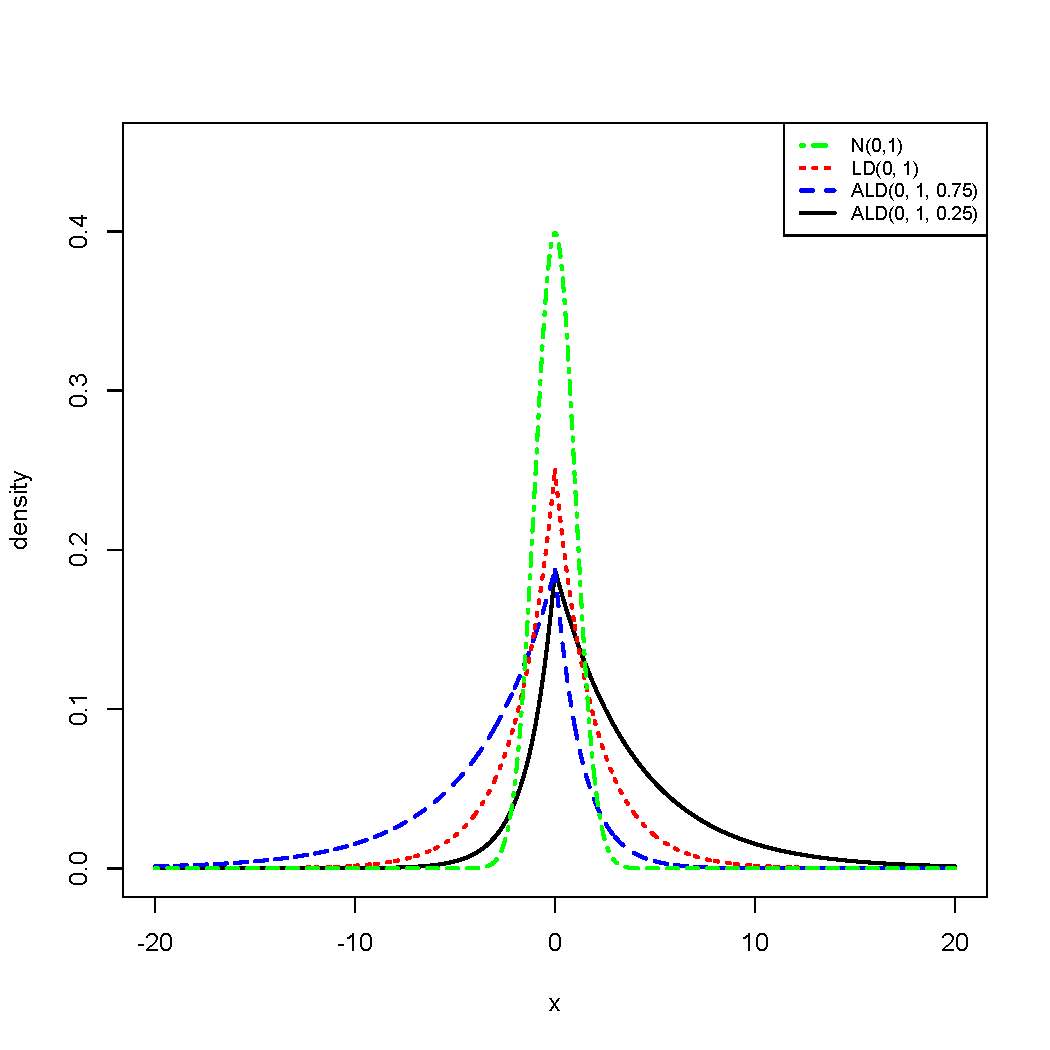
\includegraphics[width=0.6\textwidth]{ald_ld_normal.pdf}
% \end{figure}

\subsection{Scenario one}
In this scenario data are generated using Model (\ref{eqn:joint}). Choose the $\tau=$ {\bf 0.25} for the ALD distribution.


% qt25, median then normal fit
% latex table generated in R 3.1.2 by xtable 1.7-4 package
% Mon Jul 27 22:17:34 2015
\begin{table}[H]
\centering
\caption{Summary of inference result for Scenario One}
\begin{tabular}{rccccccccccc}
\hline
& \multicolumn{3}{c}{QRJM ($\tau=0.25$)} & &\multicolumn{3}{c}{QRJM ($\tau=0.5$)} & & \multicolumn{3}{c}{LMJM}\\
\hline
 & bias & se & MSE & & bias & se & MSE & & bias & se & MSE \\
 \cline{2-4}  \cline{6-8}  \cline{10-12}
  alpha1 & -0.07 & 0.08 & 0.01 & & -0.08 & 0.09 & 0.01 & & 0.33 & 0.38 & 0.25 \\
  alpha2 & 0.03 & 0.90 & 0.81 & & -0.13 & 0.58 & 0.35 & & -0.61 & 0.67 & 0.82 \\
  beta[1] & 0.02 & 0.13 & 0.02 & & 1.75 & 0.17 & 3.08 & & 2.17 & 0.71 & 5.21 \\
  beta[2] & -0.01 & 0.09 & 0.01 & & -0.01 & 0.12 & 0.02 & & -0.02 & 0.17 & 0.03 \\
  c & 0.08 & 0.18 & 0.04 & & 0.08 & 0.19 & 0.04 & & -0.19 & 0.21 & 0.08 \\
  delta[1] & 0.00 & 0.09 & 0.01 & & 0.00 & 0.10 & 0.01 & & 0.17 & 0.20 & 0.07 \\
  delta[2] & -0.01 & 0.07 & 0.01 & & -0.01 & 0.09 & 0.01 & & 0.06 & 0.31 & 0.10 \\
  gamma[1] & 0.08 & 0.04 & 0.01 & & 0.08 & 0.04 & 0.01 & & -0.00 & 0.06 & 0.00 \\
  gamma[2] & -0.08 & 0.05 & 0.01 & & -0.08 & 0.04 & 0.01 & & 0.00 & 0.06 & 0.00 \\
  sigma & 0.00 & 0.03 & 0.00 & & -0.31 & 0.02 & 0.10 & & - & - & - \\
   \hline
\end{tabular}
\end{table}

\begin{figure}[H]
\centering
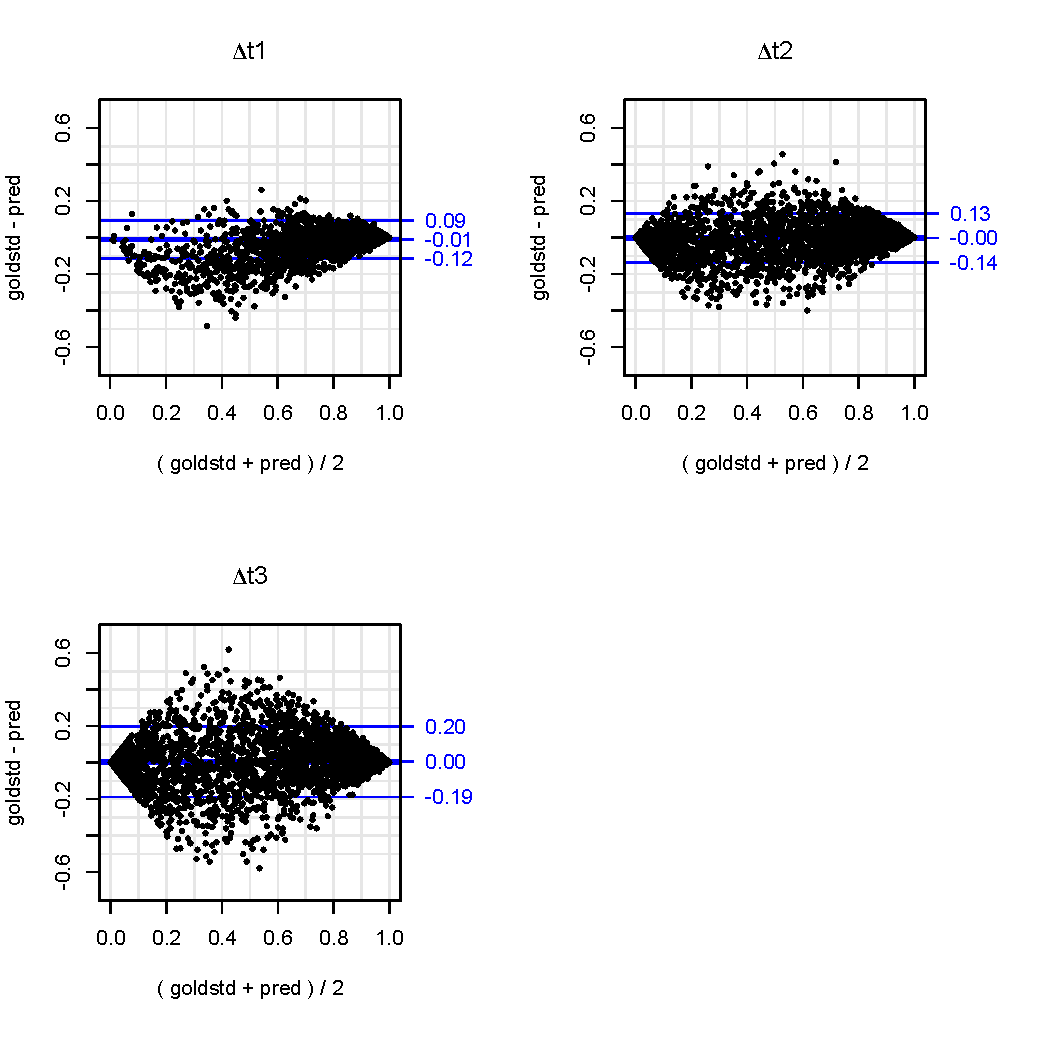
\includegraphics[width=0.5\textwidth]{ba_qt25data_qt25fit.pdf}
\caption{BA plot: data fitted using QRJM model with $\tau=0.25$}
\end{figure}

\begin{figure}[H]
\centering
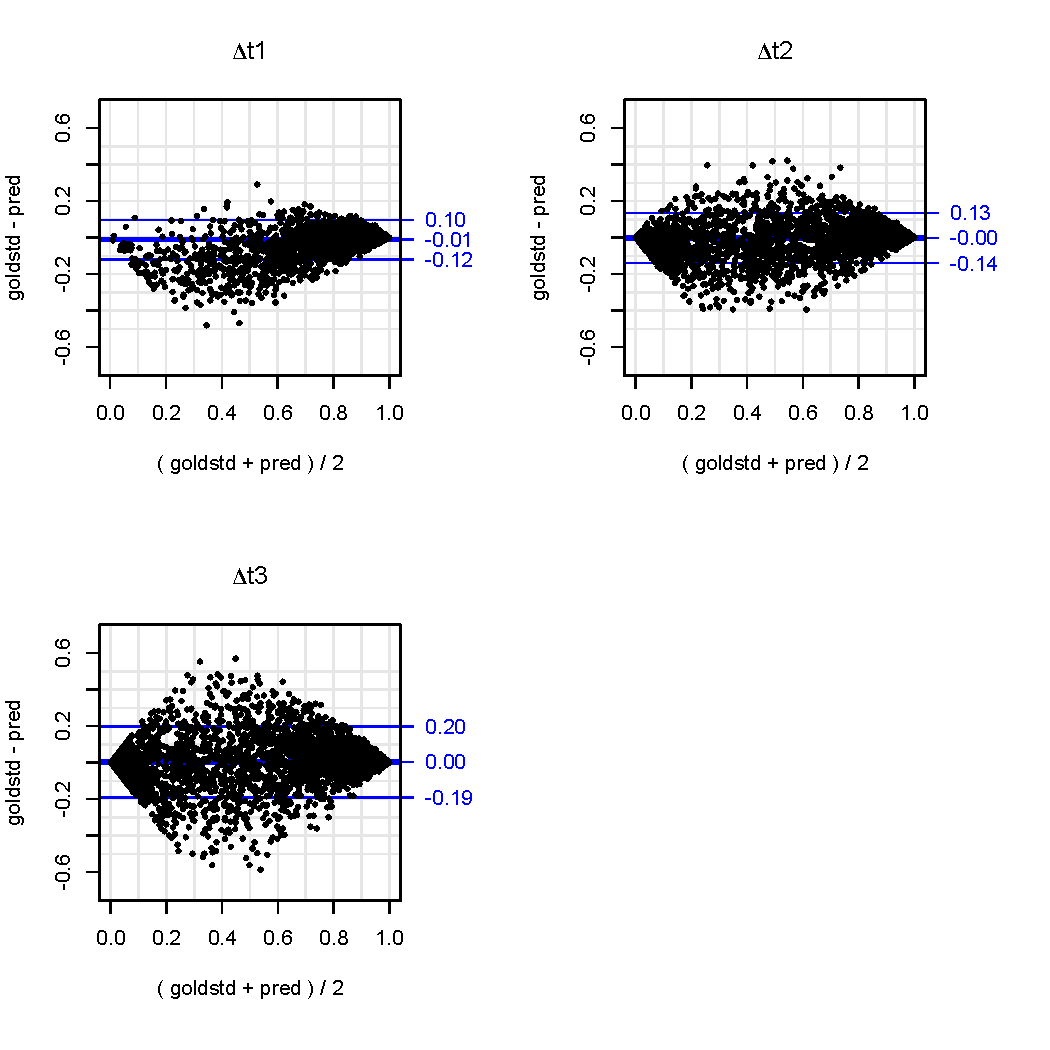
\includegraphics[width=0.5\textwidth]{ba_qt25data_medianfit.pdf}
\caption{BA plot: data fitted using QRJM model with $\tau=0.50$}
\end{figure}

\begin{figure}[H]
\centering
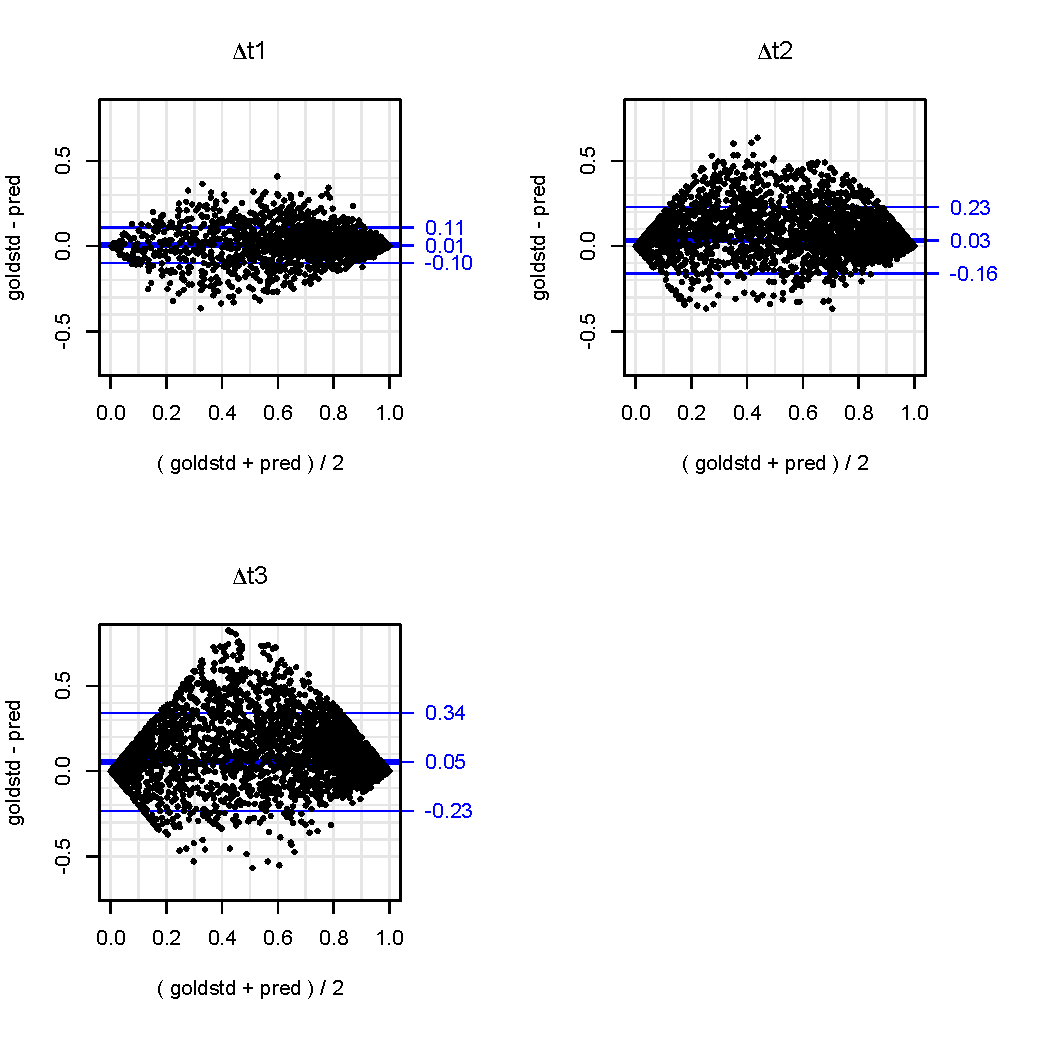
\includegraphics[width=0.5\textwidth]{ba_qt25data_meanfit.pdf}
\caption{BA plot: data fitted using LMJM}
\end{figure}



\subsection{Scenario two}
In this scenario data are generated using Model (\ref{eqn:joint}). Choose $\tau= ${\bf 0.5} for the ALD distribution.


% qt25, median then normal fit
% latex table generated in R 3.1.2 by xtable 1.7-4 package
% Mon Jul 27 22:39:39 2015
% \begin{table}[H]
% \centering
% \caption{Summary of inference result for Scenario Two}
% \begin{tabular}{rccccccccccc}
% \hline
% & \multicolumn{3}{c}{QRJM ($\tau=0.25$)} & &\multicolumn{3}{c}{QRJM ($\tau=0.5$)} & & \multicolumn{3}{c}{LMJM}\\
% \hline
%  & bias & se & MSE & & bias & se & MSE & & bias & se & MSE \\
%  \cline{2-4}  \cline{6-8}  \cline{10-12}
%   alpha1 & -0.09 & 0.09 & 0.02 & & -0.07 & 0.09 & 0.01 & & 0.49 & 0.49 & 0.48 \\
%   alpha2 & -0.35 & 0.37 & 0.26 & & 0.23 & 0.76 & 0.63 & & -0.05 & 0.55 & 0.31 \\
%   beta[1] & -1.42 & 0.15 & 2.03 & & -0.00 & 0.11 & 0.01 & & -0.43 & 0.39 & 0.33 \\
%   beta[2] & -0.01 & 0.10 & 0.01 & & 0.00 & 0.08 & 0.01 & & -0.00 & 0.12 & 0.01 \\
%   c & 0.11 & 0.17 & 0.04 & & 0.10 & 0.17 & 0.04 & & -0.09 & 0.20 & 0.05 \\
%   delta[1] & -0.01 & 0.09 & 0.01 & & 0.00 & 0.07 & 0.01 & & 0.20 & 0.16 & 0.07 \\
%   delta[2] & -0.01 & 0.07 & 0.01 & & -0.00 & 0.06 & 0.00 & & -0.10 & 0.21 & 0.05 \\
%   gamma[1] & 0.09 & 0.04 & 0.01 & & 0.08 & 0.04 & 0.01 & & 0.00 & 0.05 & 0.00 \\
%   gamma[2] & -0.09 & 0.04 & 0.01 & & -0.08 & 0.04 & 0.01 & & -0.01 & 0.06 & 0.00 \\
%   sigma & 0.26 & 0.05 & 0.07 & & 0.01 & 0.04 & 0.00 & & - & - & - \\
%    \hline
% \end{tabular}
% \end{table}

\begin{table}[H]
\centering
\caption{Summary table of inference result}
\begin{tabular}{rccccccc}
\hline
& \multicolumn{3}{c}{QRJM ($\tau=0.5$)} & & \multicolumn{3}{c}{LMJM}\\
\hline
 & bias & se & MSE & & bias & se & MSE \\
 \cline{2-4}  \cline{6-8}
alpha1 & -0.07 & 0.09 & 0.01 & & 0.49 & 0.49 & 0.48 \\
  alpha2 & 0.23 & 0.76 & 0.63 & & -0.05 & 0.55 & 0.31 \\
  beta[1] & -0.00 & 0.11 & 0.01 & & -0.43 & 0.39 & 0.33 \\
  beta[2] & 0.00 & 0.08 & 0.01 & & -0.00 & 0.12 & 0.01 \\
  c & 0.10 & 0.17 & 0.04 & & -0.09 & 0.20 & 0.05 \\
  delta[1] & 0.00 & 0.07 & 0.01 & & 0.20 & 0.16 & 0.07 \\
  delta[2] & -0.00 & 0.06 & 0.00 & & -0.10 & 0.21 & 0.05 \\
  gamma[1] & 0.08 & 0.04 & 0.01 & & 0.00 & 0.05 & 0.00 \\
  gamma[2] & -0.08 & 0.04 & 0.01 & & -0.01 & 0.06 & 0.00 \\
  sigma & 0.01 & 0.04 & 0.00 & & - & - & - \\
   \hline
\end{tabular}
\end{table}


\begin{figure}[H]
\centering
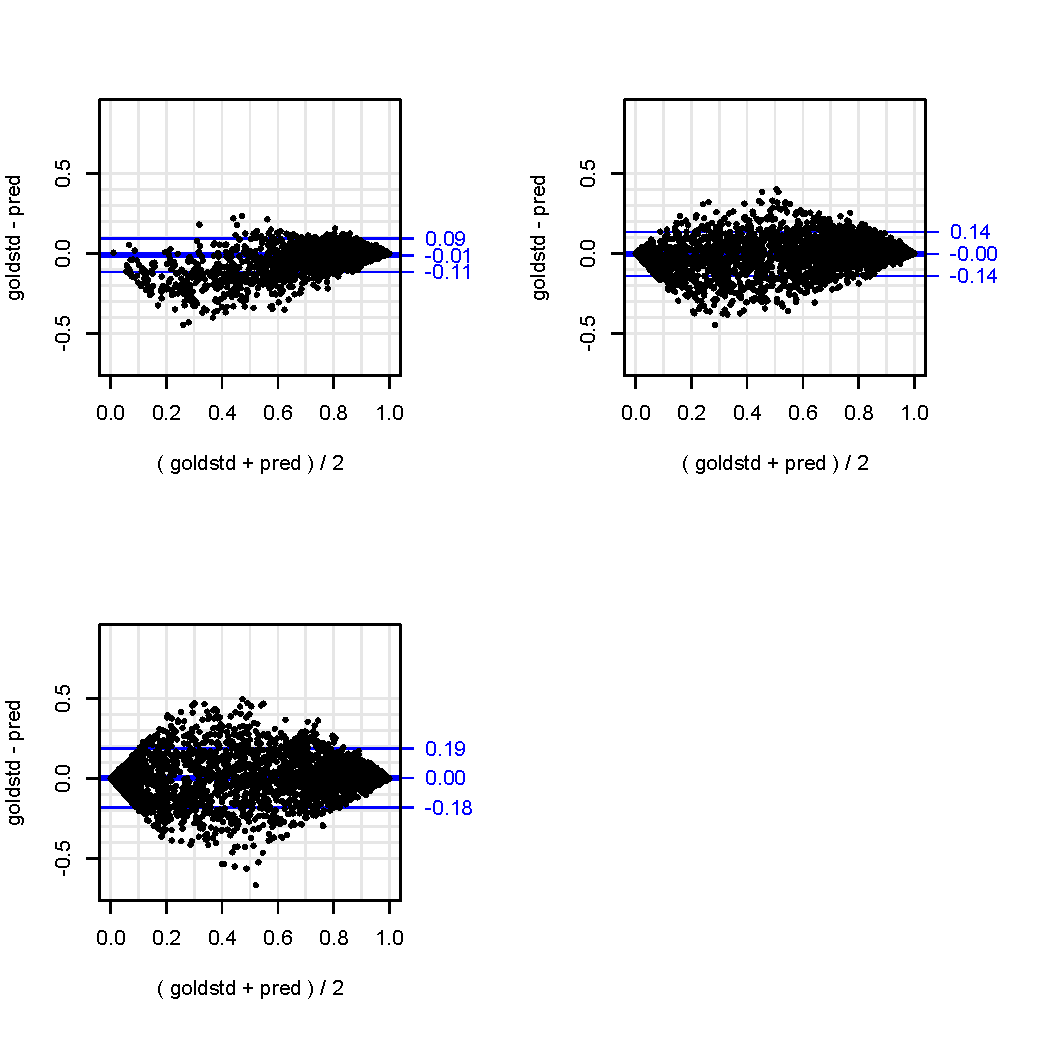
\includegraphics[width=0.5\textwidth]{ba_qt50data_medianfit.pdf}
\caption{BA plot: data fitted with JM using QR model with $\tau=0.5$}
\end{figure}

\begin{figure}[H]
\centering
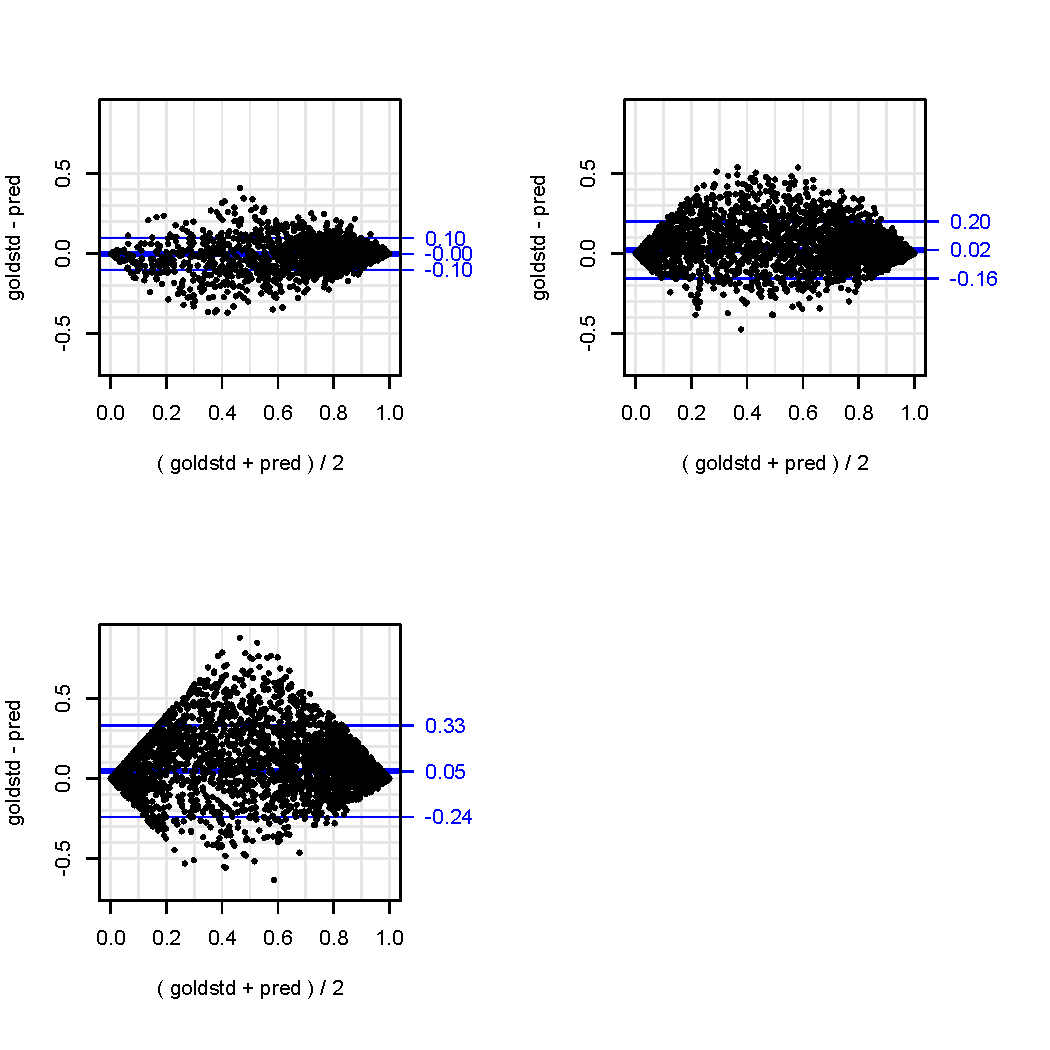
\includegraphics[width=0.5\textwidth]{ba_qt50data_meanfit.pdf}
\caption{BA plot: data fitted with JM using linear mixed model}
\end{figure}




\subsection{Scenario three}
In this scenario data are generated using Model (\ref{eqn:joint}), but the random error follows standard normal distribution instead of ALD.



% median then mean fit
% latex table generated in R 3.1.2 by xtable 1.7-4 package
% Sun Aug  2 20:33:08 2015
\begin{table}[H]
\centering
\caption{Summary table of inference result}
\begin{tabular}{rccccccc}
\hline
& \multicolumn{3}{c}{QRJM ($\tau=0.5$)} & & \multicolumn{3}{c}{LMJM}\\
\hline
 & bias & se & MSE & & bias & se & MSE \\
 \cline{2-4}  \cline{6-8}
alpha1 & -0.10 & 0.07 & 0.01 & & 0.52 & 0.50 & 0.52 \\
  alpha2 & -0.04 & 0.49 & 0.24 & & 1.24 & 1.06 & 2.65 \\
  beta[1] & 0.01 & 0.07 & 0.01 & & -0.23 & 0.30 & 0.14 \\
  beta[2] & 0.00 & 0.05 & 0.00 & & 0.00 & 0.06 & 0.00 \\
  c & 0.13 & 0.16 & 0.04 & & 0.28 & 0.43 & 0.26 \\
  delta[1] & 0.00 & 0.05 & 0.00 & & 0.10 & 0.12 & 0.03 \\
  delta[2] & -0.00 & 0.04 & 0.00 & & -0.27 & 0.30 & 0.17 \\
  gamma[1] & 0.09 & 0.05 & 0.01 & & 0.02 & 0.07 & 0.01 \\
  gamma[2] & -0.10 & 0.05 & 0.01 & &  -0.03 & 0.07 & 0.01 \\
  sigma & - & - & - & & 0.33 & 0.24 & 0.17 \\
   \hline
\end{tabular}
\end{table}



\begin{figure}[H]
\centering
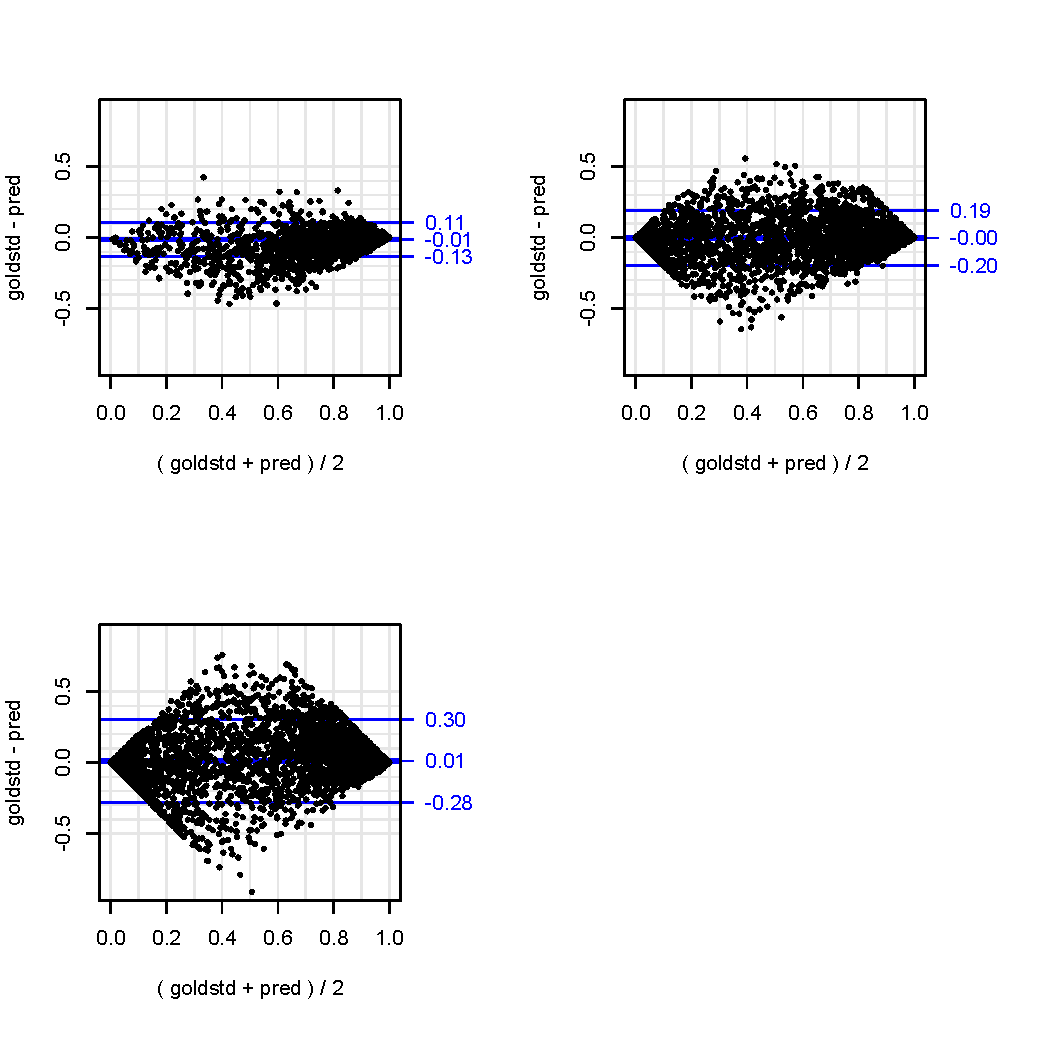
\includegraphics[width=0.5\textwidth]{ba_normdata_meanfit.pdf}
\caption{BA plot: data fitted with JM using linear mixed model}
\end{figure}

\begin{figure}[H]
\centering
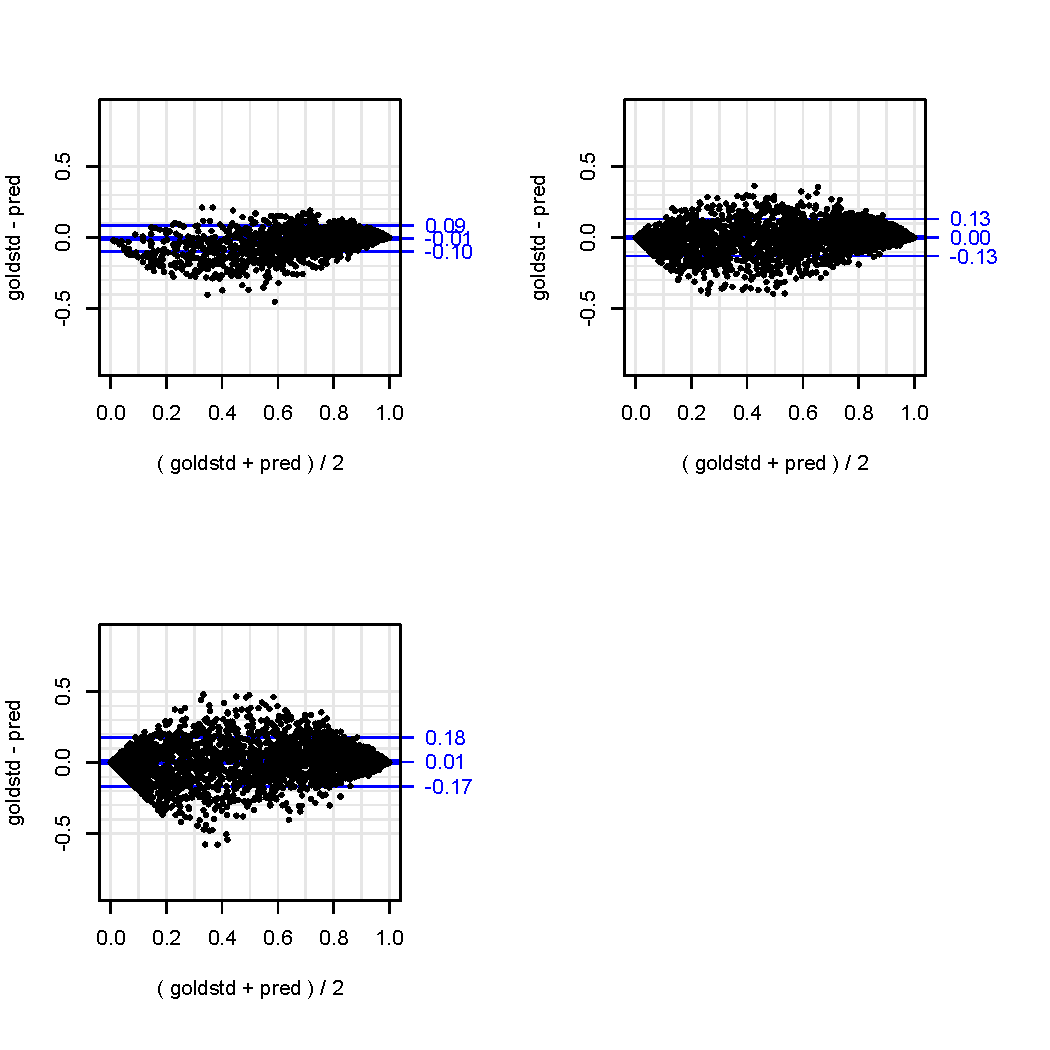
\includegraphics[width=0.5\textwidth]{ba_normdata_medianfit.pdf}
\caption{BA plot: data fitted with JM using QR model with $\tau=0.5$}
\end{figure}





\subsection{Summary table -- predictions}

\begin{table}[H]
\centering
\caption{MSE and bias of the predictions of survival probabilities from two models ($\Delta t_1<\Delta t_2<\Delta t_3$)}
\begin{tabular}{ccccccc}
\hline
Scenario & & \multicolumn{2}{c}{LMJM} & & \multicolumn{2}{c}{QRJM} \\
\cline{3-4}\cline{6-7}
 & & MSE & Bias & & MSE & Bias \\
\hline
\multirow{3}{*}{1} & $\Delta t_1$ & 0.003 & -0.005 & & 0.003 & 0.011 \\
& $\Delta t_2$ & 0.011 & -0.033 & & 0.005 & 0.002 \\
& $\Delta t_3$ & 0.024 & -0.053 & & 0.009 & -0.005 \\
\hline
\multirow{3}{*}{2} & $\Delta t_1$ & 0.002 & 0.003 & & 0.003 & 0.010 \\
& $\Delta t_2$ & 0.008 & -0.023 & & 0.005 & 0.002 \\
& $\Delta t_3$ & 0.022 & -0.046 & & 0.009 & -0.004 \\
\hline
\multirow{3}{*}{3} & $\Delta t_1$ & 0.004 & 0.013 & & 0.002 & 0.006 \\
& $\Delta t_2$ & 0.009 & 0.002 & & 0.004 & -0.001 \\
& $\Delta t_3$ & 0.022 & -0.012 & & 0.007 & -0.005 \\
\hline
\end{tabular}
\end{table}




\subsection{Comments}
\begin{enumerate}
\item In both model settings, the accuracy (in terms of MSE and bias) of predictions decreases as $\Delta t$ increases, which makes sense as it's more difficult to accurately predict the survival for longer time in the future since there are more variabilities and uncertainty.
\item QRJM and LMJM perform closely in predicting the survival probabilities when $\Delta t$ is smaller but when $\Delta t$ increases QRJM will outperform LMJM based on the BA plots, bias and MSE.
\end{enumerate}












\end{document}